\documentclass[12pt, a4paper, oneside]{book}

% Fonts
\usepackage[]{opensans}
\usepackage[T1]{fontenc}
\usepackage[utf8]{inputenc}

% Paragraphs
\setlength{\parindent}{0pt}
\setlength{\parskip}{6pt plus 2pt minus 1pt}

% Margins
\usepackage[margin=1in]{geometry}

% Images
\usepackage{graphicx}
\usepackage{float}

% Source code
\usepackage{listings}
\usepackage{xcolor}

% Source code formatting
\lstset{
	backgroundcolor=\color[rgb]{0.95,0.95,0.95},
	basicstyle=\footnotesize,
	language=Python,
	aboveskip=1em,
	belowskip=1em,
}

% Headers and footers
\pagestyle{plain}

% Urls
\usepackage{hyperref}

% Equations
\usepackage{amsmath}


\begin{document}

\title{At full speed with Python}
\author{João Ventura}
\date{v0.1}

\maketitle

{
	\setcounter{tocdepth}{2}
	\tableofcontents
}

\chapter{Introduction}\label{introduction}

This book aims to teach the basics of the Python programming language using a practical approach. Its method is quite basic though: after a simple introduction to each topic, the reader is invited to learn by solving the proposed exercises.

These exercises have been used extensively in my web development and distributed computing classes at the Superior School of Technology of Setúbal. With these exercises, most students are up to speed with Python in less than a month. In fact, students of the distributed computing course, taught in the second year of the software engineering degree, become familiar with Python's syntax in two weeks and are able to implement a distributed client-server application with sockets in the third week.

This book is divided in the following chapters: in chapter \ref{installation} I will provide the basic installation instructions and execution of the Python interpreter. In chapter \ref{basic-datatypes} we will talk about the most basic data types, numbers and strings. In chapter \ref{functions} we will start tinkering with functions, and in chapter \ref{loops} the topic is about "loops". In chapter \ref{dictionaries} we will work with dictionaries and finally, in chapter \ref{classes} we will finish the book with some exercises about classes and object oriented programming.

Please note that this book is a work in progress and, as such, may contain quite a few spelling errors that may be corrected in the future. However it is made available as it is so it can be useful to anyone who wants to use it. I sincerely hope you can get something good through it.

The source of this book is made available in github (check it at \url{https://github.com/joaoventura/full-speed-python}) so I welcome any pull requests to correct misspellings, suggest new exercises or to provide clarification of the current content.

All the best,

João Ventura - Adjunct Professor at the Escola Superior de Tecnologia de Setúbal.

\chapter{Installation}\label{installation}

In this chapter we will install and run the Python interpreter in your local computer.

\section{Installing on Windows}

\begin{enumerate}

\item Download the latest python 3 release for Windows on \url{https://www.python.org/downloads/windows/} and execute the installer. At the time of writing, this is Python 3.6.4.

\item Make sure that the "Install launcher for all users" and "Add Python to PATH" settings are selected and choose "Customize installation".

\begin{figure}[H]
	\centering
  	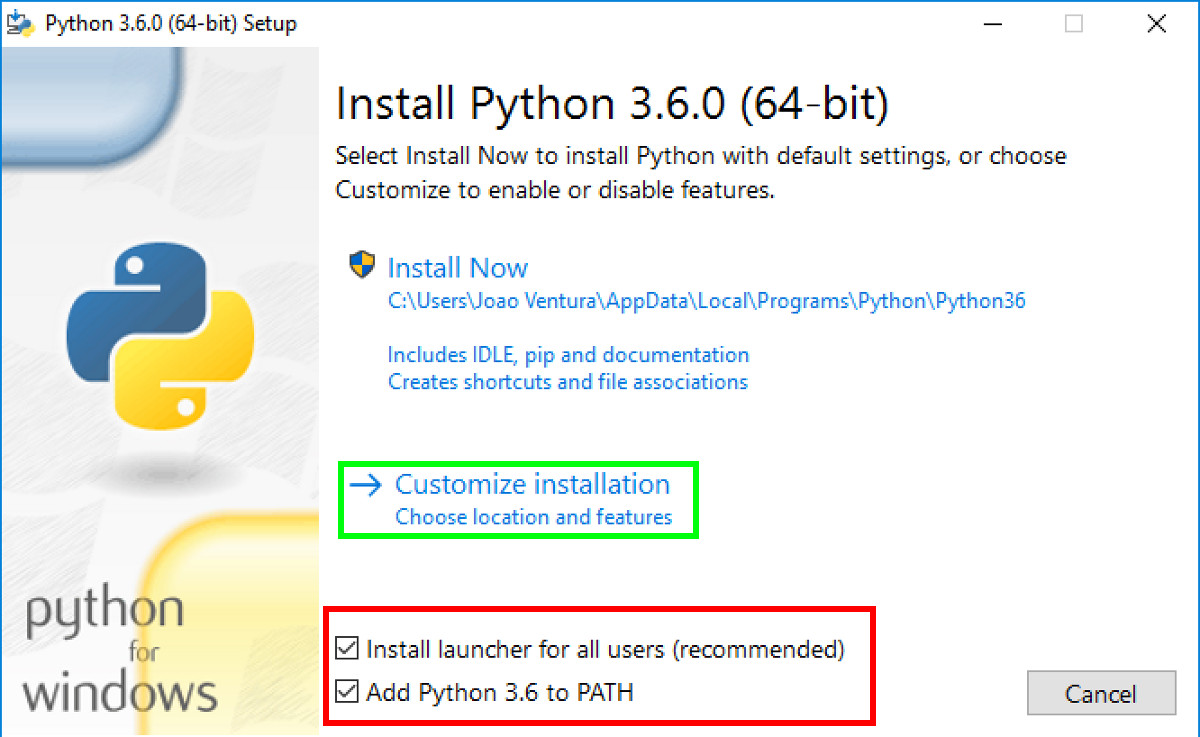
\includegraphics[width=0.6\textwidth]{images/python_windows.jpg}
\end{figure}

\item In the next screen "Optional Features", you can install everything, but it is essential to install "pip" and "pylauncher (for all users)". Pip is the python package manager that allows you to install several python packages and libraries.

\item In the Advanced Options, make sure that you select "Add Python to environment variables". Also, I suggest that you change the install location to something like C:{\textbackslash}Python36{\textbackslash} as it will be easier for you to find the python installation if something goes wrong.

\begin{figure}[H]
	\centering
  	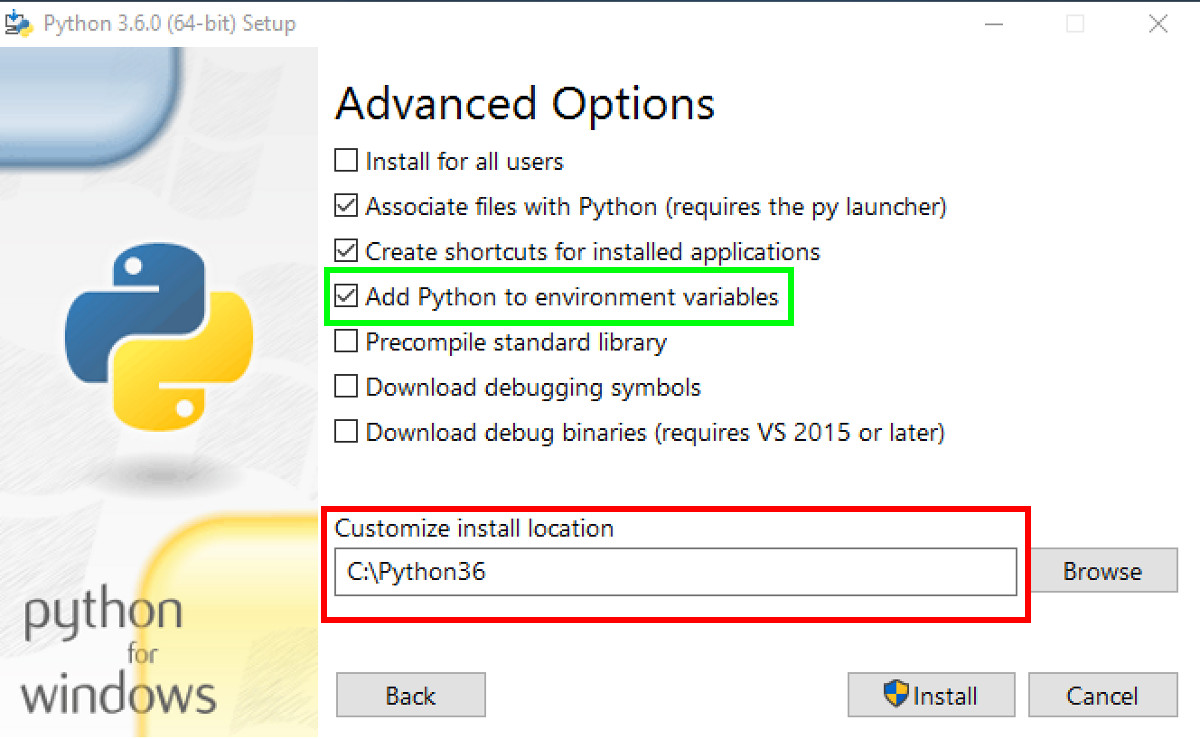
\includegraphics[width=0.6\textwidth]{images/python_windows2.jpg}
\end{figure}

\item Finally, allow python to use more than 260 characters on the file system by selecting "Disable path length limit" and close the installation dialog.

\begin{figure}[H]
	\centering
  	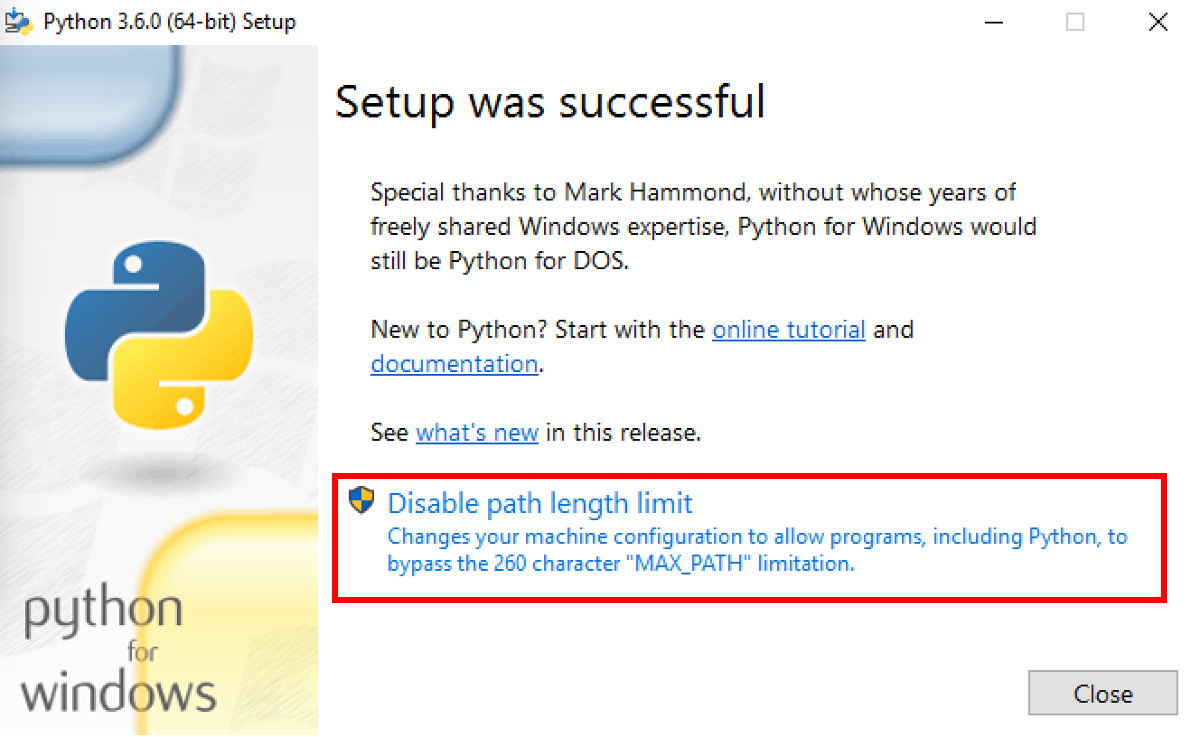
\includegraphics[width=0.6\textwidth]{images/python_windows3.jpg}
\end{figure}

\item Now, open the command line (cmd) and execute "python" or "python3". If everything was correctly installed, you should see the python REPL. The REPL (from Read, Evaluate, Print and Loop) is a environment that you can use to program small snippets of python code. Execute \textit{exit()} to exit.

\begin{figure}[H]
	\centering
  	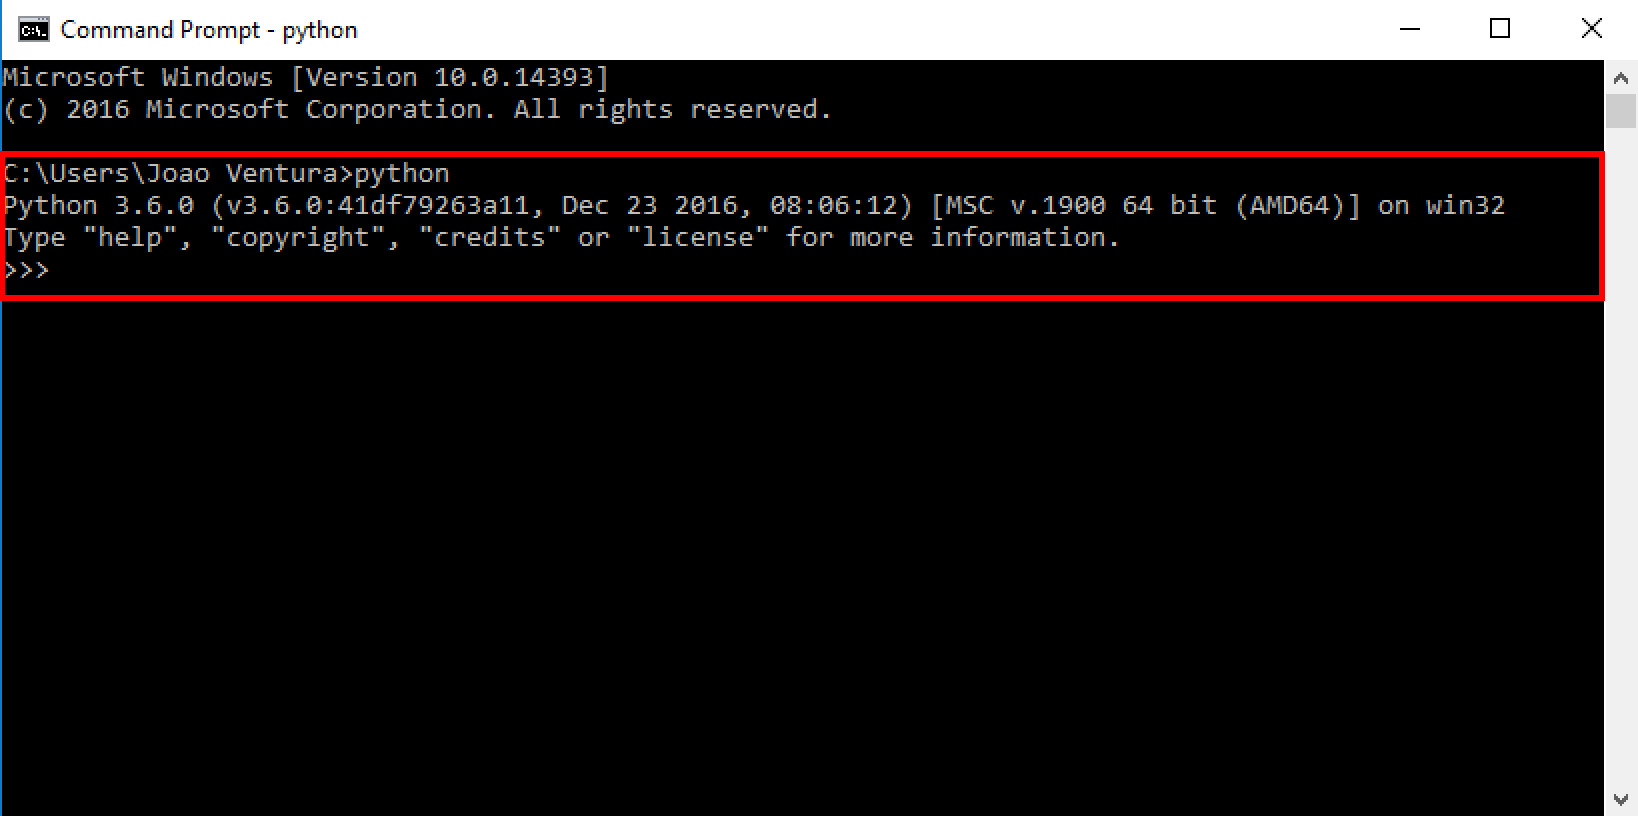
\includegraphics[width=0.62\textwidth]{images/python_windows4.jpg}
\end{figure}

\end{enumerate}

\section{Installing on macOS}

You can download the latest macOS binary releases from \url{https://www.python.org/downloads/mac-osx/}. Make sure you download the latest Python 3 release (3.6.4 at the time of writing). You can also use Homebrew, a package manager for macOS (\url{https://brew.sh/}). To install the latest Python 3 release with Homebrew, just do "\texttt{brew install python3}" on your terminal.

\begin{figure}[H]
	\centering
  	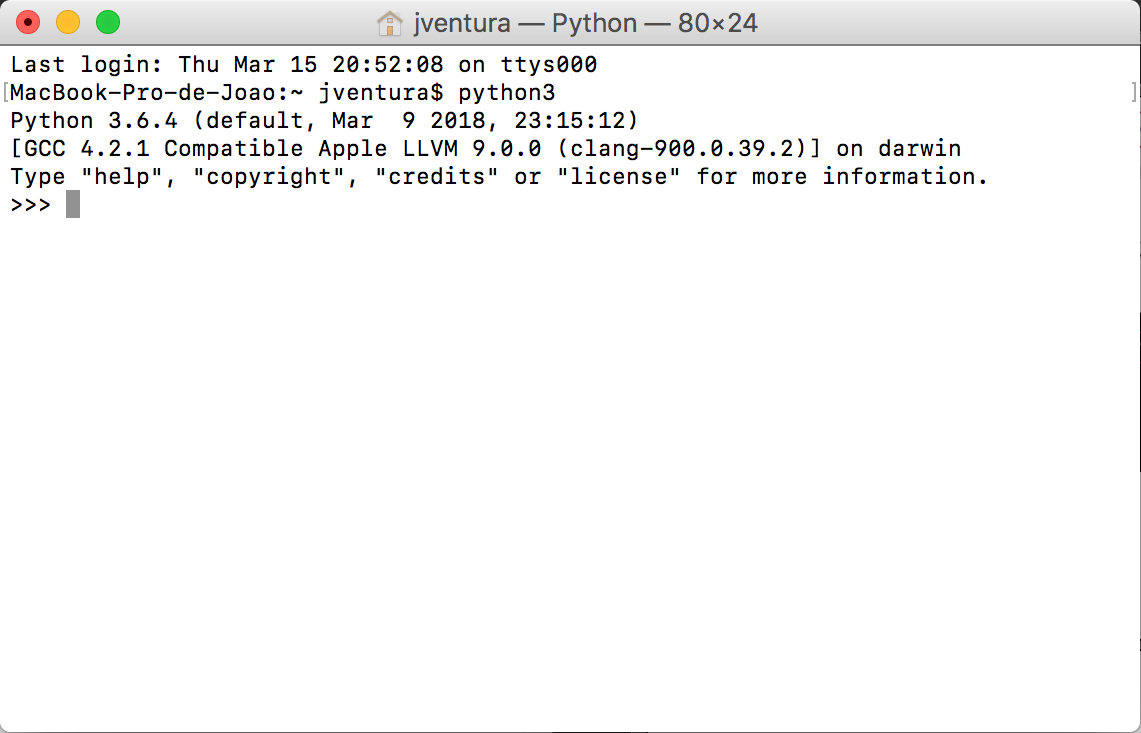
\includegraphics[width=0.62\textwidth]{images/python_macos.png}
\end{figure}

Finally, open the terminal, execute $python3$ and you should see the Python REPL as above. Press Ctrl+D or write $exit()$ to leave the REPL.

\section{Installing on Linux}

For Linux, you can download the latest Python 3 binary releases from \url{https://www.python.org/downloads/linux/} or use your package manager to install it. To make sure you have python 3 installed on your system, run $python3$ in your terminal.

\begin{figure}[H]
	\centering
  	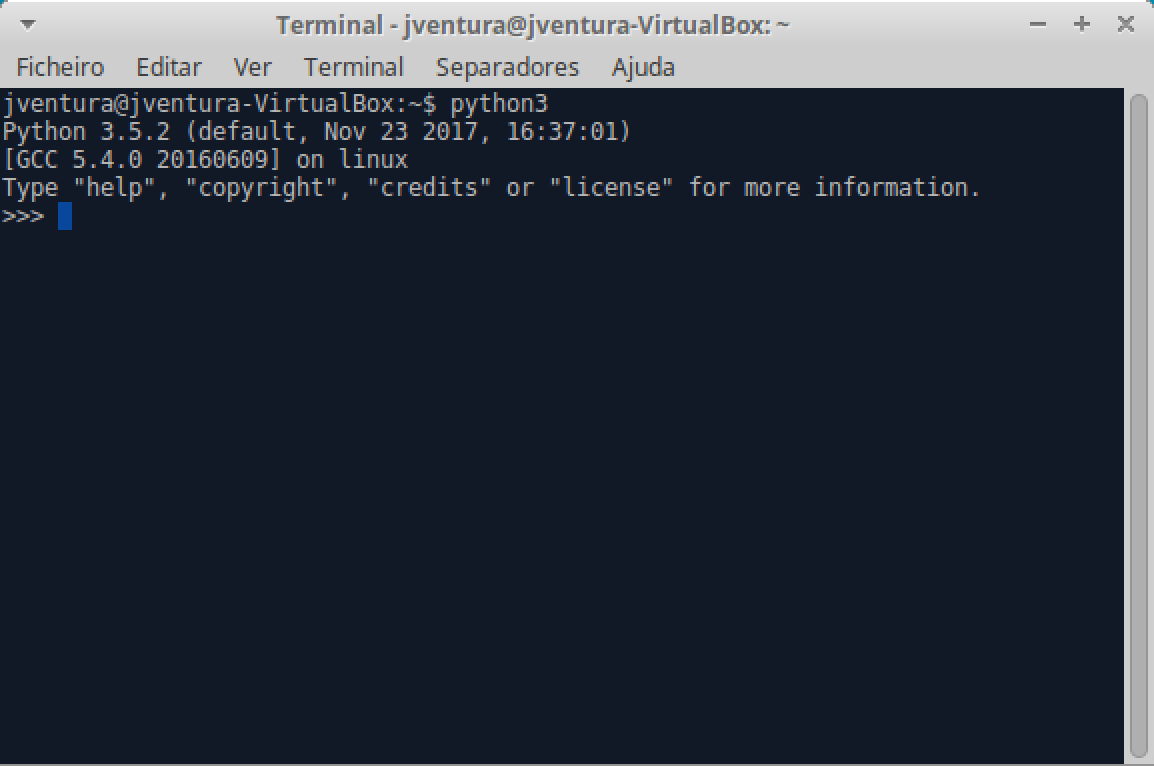
\includegraphics[width=0.62\textwidth]{images/python_linux.png}
\end{figure}

Finally, open the terminal, execute $python3$ and you should see the Python REPL as above. Press Ctrl+D or write $exit()$ to leave the REPL.
\chapter{Basic datatypes}\label{basic-datatypes}

In this chapter we will work with the most basic datatypes, numbers, strings and lists. Start your Python REPL and write the following on it:

\begin{lstlisting}
>>> a = 2
>>> type(a)
<class 'int'>
>>> b = 2.5
>>> type(b)
<class 'float'>
\end{lstlisting}

Basically, you are declaring two variables (named "a" and "b") which will hold some numbers: variable "a" is an integer number while variable "b" is a real number. We can now use our variables or any other numbers to do some calculations:

\begin{lstlisting}
>>> a + b
4.5
>>> (a + b) * 2
9.0
>>> 2 + 2 + 4 - 2/3
7.333333333333333
\end{lstlisting}

Python also has support for string datatypes. Strings are sequences of characters (like words) and can be defined using single or double quotes:

\begin{lstlisting}
>>> hi = "hello"
>>> hi
'hello'
>>> bye = 'goodbye'
>>> bye
'goodbye'
\end{lstlisting}

You can add strings to concatenate them but you can not mix different datatypes, such as strings and integers.

\begin{lstlisting}
>>> hi + "world"
'helloworld'
>>> "Hello" + 3
Traceback (most recent call last):
  File "<stdin>", line 1, in <module>
TypeError: must be str, not int
\end{lstlisting}

However, multiplication seems to work as repetition:

\begin{lstlisting}
>>> "Hello" * 3
'HelloHelloHello'
\end{lstlisting}

Finally, Python also supports the list datatype. Lists are data structures that allows us to group some values. Lists can have values of several types and you can also mix different types within the same list although usually all values are usually of the same datatype. 

Lists are created by starting and ending with square brackets and separated by commas. The values in a list can be accessed by its position where 0 is the index of the first value:

\begin{lstlisting}
>>> l = [1, 2, 3, 4, 5]
>>> l[0]
1
>>> l[1]
2
\end{lstlisting}

Can you access the number 4 in the previous list?

Sometimes you want just a small portion of a list, a sublist. Sublists can be retrieved using a technique called \textit{slicing}, which consists on using the start and end indexes on the sublist:

\begin{lstlisting}
>>> l = ['a', 'b', 'c', 'd', 'e']
>>> l[1:3]
['b', 'c']
\end{lstlisting}

Finally, there's also some arithmetic that you can do on lists, like adding two lists together or repeating the contents of a list.

\begin{lstlisting}
>>> [1,2] + [3,4]
[1, 2, 3, 4]
>>> [1,2] * 2
[1, 2, 1, 2]
\end{lstlisting}


\section{Exercises with numbers}

\begin{enumerate}

\item Try the following mathematical calculations and guess what is happening: $(3 / 2)$, $(3 // 2)$, $(3 \% 2)$, $(3**2)$.

Suggestion: check the Python library reference at \url{https://docs.python.org/3/library/stdtypes.html#numeric-types-int-float-complex}.

\item Calculate the average of the following sequences of numbers: (2, 4), (4, 8, 9), (12, 14/6, 15)

\item The volume of a sphere is given by $4/3\pi r^3$. Calculate the volume of a sphere of radius 5. Suggestion: create a variable named "pi" with the value of 3.1415.

\item Use the module operator (\%) to check which of the following numbers is even or odd: (1, 5, 20, 60/7).

Suggestion: the remainder of $x/2$ is always zero when $x$ is even.

\item Find some values for $x$ and $y$ such that $x < 1/3 < y$ returns "True" on the Python REPL. Suggestion: try $0 < 1/3 < 1$ on the REPL.

\end{enumerate}

\section{Exercises with strings}

Using the Python documentation on strings (\url{https://docs.python.org/3/library/string.html)}, solve the following exercises:

\begin{enumerate}

\item Initialize the string "abc" on a variable named "s":
\begin{enumerate}
\item Use a function to get the length of the string.
\item Write the necessary sequence of operations to transform the string "abc" in "aaabbbccc". Suggestion: Use string concatenation and string indexes.
\end{enumerate}

\item Initialize the string "aaabbbccc" on a variable named "s":
\begin{enumerate}
\item Use a function that allows you to find the first occurence of "b" in the string, and the first occurence of "ccc".
\item Use a function that allows you to replace all occurences of "a" to "X", and then use the same function to change only the first occurence of "a" to "X".
\end{enumerate}

\item Starting from the string "aaa bbb ccc", what sequences of operations do you need to arrive at the following strings? You can find the "replace" function.
\begin{enumerate}
\item "AAA BBB CCC"
\item "AAA bbb CCC"
\end{enumerate}

\end{enumerate}

\section{Exercises with lists}

Create a list named "l" with the following values ([1, 4, 9, 10, 23]). Using the Python documentation about lists (\url{https://docs.python.org/3.5/tutorial/introduction.html#lists}) solve the following exercises:

\begin{enumerate}

\item Using list slicing get the sublists [4, 9] and [10, 23].

\item Append the value 90 to the end of the list "l". Check the difference between list concatenation and the "append" method.

\item Calculate the average value of all values on the list. You can use the "sum" and "len" functions.

\item Remove the sublist [4, 9].

\end{enumerate}

\chapter{Modules and functions}\label{functions}

In this chapter we will talk about modules and functions. A function is a block of code that is used to perform a single action. A module is a Python file containing variables, functions and many more things. 

Start up your Python REPL and let's use the "math" module which provides access to mathematical functions:

\begin{lstlisting}
>>> import math
>>> math.cos(0.0)
1.0
>>> math.radians(275)
4.799655442984406
\end{lstlisting}

Functions are sequences of instructions that are executed when the function is invoked. The following defines the "do\_hello" function that prints two messages when invoked:

\begin{lstlisting}
>>> def do_hello():
...     print("Hello")
...     print("World")
... 
>>> do_hello()
Hello
World
\end{lstlisting}

Make sure that you insert a tab before both print expressions in the previous function. Tabs and spaces in Python are relevant and define that a block of code is somewhat dependent on a previous instruction. For instance, the print expressions are "inside" the "do\_hello" function therefore must have a tab.

Functions can also receive parameters a return values (using the "return" keyword):

\begin{lstlisting}
>>> def add_one(val):
...     print("Function got value", val)
...     return val + 1
... 
>>> value = add_one(1)
Function got value 1
>>> value
2
\end{lstlisting}

\section{Exercises with the math module}

Use the Python documentation about the math module (\url{https://docs.python.org/3/library/math.html}) to solve the following exercises:

\begin{enumerate}

\item Find the greatest common divisor of the following pairs of numbers: (15, 21), (152, 200), (1988, 9765). 

\item Compute the base-2 logarithm of the following numbers: 0, 1, 2, 6, 9, 15.

\item Use the "input" function to ask the user for a number and show the result of the sine, cosine and tangent of the number. Make sure that you convert the user input from string to a number (use the int() or the float() function).

\end{enumerate}

\section{Exercises with functions}

\begin{enumerate}

\item Implement the "add2" function that receives two numbers as arguments and returns the sum of the numbers. Then implement the "add3" function that receives and sums 3 parameters.

\item Implement a function that returns the greatest of two numbers given as parameters. Use the "if" statement to compare both numbers: \url{https://docs.python.org/3/tutorial/controlflow.html#if-statements}.

\item Implement a function named "is\_divisible" that receives two parameters (named "a" and "b") and returns true if "a" can be divided by "b" or false otherwise. A number is divisible by another when the remainder of the division is zero. Use the modulo operator ("\%").

\item Create a function named "average" that computes the average value of a list passed as parameter to the function. Use the "sum" and "len" functions.

\end{enumerate}

\section{Recursive functions}

In computer programming, a recursive function is simply a function that calls itself. For instance take the factorial function.

\begin{equation}
f(x)=\begin{cases}
    1, & \text{if $x=0$}.\\
    x \times f(x-1), & \text{otherwise}.
\end{cases}
\end{equation}

As an example, take the factorial of 5:

\begin{equation}
\begin{split}
5! &= 5 \times 4! \\
    &= 5 \times 4 \times 3! \\
    &= 5 \times 4 \times 3 \times 2! \\
    &= 5 \times 4 \times 3 \times 2 \times 1 \\
    &= 120
\end{split}
\end{equation}

Basically, the factorial of 5 is 5 times the factorial of 4, etc. Finally, the factorial of 1 (or of zero) is 1 which breaks the recursion. In Python we could write the following recursive function:

\begin{lstlisting}
def factorial(x):
      if x == 0:
          return 1
      else:
          return x * factorial(x-1)
\end{lstlisting}

The trick with recursive functions is that there must be a "base" case where the recursion must end and a recursive case that iterates towards the base case. In the case of factorial we know that the factorial of zero is one, and the factorial of a number greater that zero will depend on the factorial of the previous number until it reaches zero.

\section{Exercises with recursive functions}

\begin{enumerate}

\item Implement the factorial function and test it with several different values. Cross-check with a calculator.

\item Implement a recursive function to compute the sum of the $n$ first integer numbers (where $n$ is a function parameter). Start by thinking about the base case (the sum of the first 0 integers is?) and then think about the recursive case.

\item The Fibonnaci sequence is a sequence of numbers in which each number of the sequence matches the sum of the previous two terms. Given the following recursive definition implement $fib(n)$.

\begin{equation}
fib(n)=\begin{cases}
    0, & \text{if $x=0$}.\\
    1, & \text{if $x=1$}.\\
    fib(n-1) + fib(n-2), & \text{otherwise}.
\end{cases}
\end{equation}

Check your results for the first numbers of the sequence: 0, 1, 1, 2, 3, 5, 8, 13, 21, 34, 55, 89, ...

\end{enumerate}

\chapter{Iteration and loops}\label{loops}

In this chapter we are going to explore the topics of iteration and loops. Loops are used in computer programming to automate repetitive tasks. 

In Python the most common form of iteration is the "for" loop. The "for" loop allows you to iterate over all items of a list such that you can do whatever you want with each item. For instance, let's create a list and print the square value of each element.

\begin{lstlisting}
>>> for value in [0, 1, 2, 3, 4, 5]:
...     print(value * value)
... 
0
1
4
9
16
25
\end{lstlisting}

It's quite easy but very powerful! The "for" loop is the basis of many things in programming. For instance, you already know about the "sum(list)" function which sums all the elements of a list, but here's an example using the "for" loop:

\begin{lstlisting}
>>> mylist = [1,5,7]
>>> sum = 0
>>> for value in mylist:
...     sum = sum + value
... 
>>> print(sum)
13
\end{lstlisting}

Basically, you create the variable "sum" and keep adding each value as it comes from the list. 

Sometimes, instead of the values of a list, you may need to work with the indexes themselves, i.e., not with the values, but the positions where they are in the list. Here's an example that iterates over a list and returns the indexes and the values for each index:

\begin{lstlisting}
>>> mylist = [1,5,7]
>>> for i in range(len(mylist)):
...     print("Index:", i, "Value:", mylist[i])
... 
Index: 0 Value: 1
Index: 1 Value: 5
Index: 2 Value: 7
\end{lstlisting}

You can see that we are not iterating over the list itself but iterating over the "range" of the length of the list. The range function returns a special list:

\begin{lstlisting}
>>> list(range(3))
[0, 1, 2]
\end{lstlisting}

So, when you use "range" you are not iterating over "mylist" but over a list with some numbers that you'll use as indexes to access individual values on "mylist". More about the range function in the Python docs at \url{https://docs.python.org/3/tutorial/controlflow.html#the-range-function}.

Sometimes you may need both things (indexes and values), and you can use the "enumerate" function:

\begin{lstlisting}
>>> mylist = [1,5,7]
>>> for i, value in enumerate(mylist):
...     print("Index:", i, "Value:", value)
... 
Index: 0 Value: 1
Index: 1 Value: 5
Index: 2 Value: 7
\end{lstlisting}

Remember that the first value on a Python list is always at index 0. 

Finally, we also have the "while" statement that allows us to repeat a sequence of instructions while a specified condition is true. For instance, the following example starts "n" at 10 and \textbf{while "n" is greater than 0}, it keeps subtracting 1 from "n". When "n" reaches 0, the condition "n > 0" is false, and the loop ends:

\begin{lstlisting}
>>> n = 10
>>> while n > 0:
...     print(n)
...     n = n-1
... 
10
9
8
7
6
5
4
3
2
1
\end{lstlisting}

Notice that it never prints 0...

\section{Exercises with the for loop}

For this section you may want to consult the Python docs at \url{https://docs.python.org/3/tutorial/controlflow.html#for-statements}.

\begin{enumerate}

\item Create a function "add" that receives a list as parameter and returns the sum of all elements in the list. Use the "for" loop to iterate over the elements of the list.

\item Create a function that receives a list as parameter and returns the maximum value in the list. As you iterate over the list you may want to keep the maximum value found so far in order to keep comparing it with the next elements of the list.

\item Modify the previous function such that it returns a list with the first element being the maximum value and the second being the index of the maximum value in the list. Besides keeping the maximum value found so far, you also need to keep the position where it occurred. 

\item Implement a function that returns the reverse of a list received as parameter. You may create an empty list and keep adding the values in reversed order as they come from the original list. Check what you can do with lists at \url{https://docs.python.org/3/tutorial/datastructures.html#more-on-lists}.

\item Make the function "is\_sorted" that receives a list as parameter and returns True if the list is sorted in ascending order. For instance [1, 2, 2, 3] is ordered while [1, 2, 3, 2] is not. Suggestion: you have to compare a number in the list with the next one, so you can use indexes or you need to keep the previous number in a variable as you iterate over the list.

\item Implement the function "is\_sorted\_dec" which is similar to the previous one but all items must be sorted by decreasing order.

\item Implement the "has\_duplicates" function which verifies if a list has duplicate values. You may have to use two "for" loops, where for each value you have to check for duplicates on the rest of the list.

\end{enumerate}


\section{Exercises with the while statement}

\begin{enumerate}

\item Implement a function that receives a number as parameter and prints, in decreasing order, which numbers are even and which are odd, until it reaches 0.

\begin{lstlisting}
>>> even_odd(10)
Even number: 10
Odd number: 9
Even number: 8
Odd number: 7
Even number: 6
Odd number: 5
Even number: 4
Odd number: 3
Even number: 2
Odd number: 1
\end{lstlisting}

\end{enumerate}

\chapter{Dictionaries}\label{dictionaries}

In this chapter we will work with Python dictionaries. Dictionaries are data structures that indexes values by a given key (key-value pairs). The following example shows a dictionary that indexes students ages by name.

\begin{lstlisting}
ages = {
    "Peter": 10,
    "Isabel": 11,
    "Anna": 9,
    "Thomas": 10,
    "Bob": 10,
    "Joseph": 11,
    "Maria": 12,
    "Gabriel": 10,
}

>>> print(ages["Peter"])
10
\end{lstlisting}

It is possible to iterate over the contents of a dictionary using "items", like this:

\begin{lstlisting}
>>> for name, age in ages.items():
...     print(name, age)
... 
Peter 10
Isabel 11
Anna 9
Thomas 10
Bob 10
Joseph 11
Maria 12
Gabriel 10
\end{lstlisting}

However, keys don't need to be necessarily strings and integers but can be any objects:

\begin{lstlisting}
d = {
    0: [0, 0, 0],
    1: [1, 1, 1],
    2: [2, 2, 2],
}

>>> d[2]
[2, 2, 2]
\end{lstlisting}

Even more, you can use other dictionaries as values:

\begin{lstlisting}
students = {
    "Peter": {"age": 10, "address": "Lisbon"},
    "Isabel": {"age": 11, "address": "Sesimbra"},
    "Anna": {"age": 9, "address": "Lisbon"},
}

>>> students['Peter']
{'age': 10, 'address': 'Lisbon'}
>>> students['Peter']['address']
'Lisbon'
\end{lstlisting}

This is quite useful to structure hierarchical information. 

\section{Exercises with dictionaries}

Use the Python documentation at \url{https://docs.python.org/3/library/stdtypes.html#mapping-types-dict} to solve the following exercises.

Take the following Python dictionary:

\begin{verbatim}
ages = {
    "Peter": 10,
    "Isabel": 11,
    "Anna": 9,
    "Thomas": 10,
    "Bob": 10,
    "Joseph": 11,
    "Maria": 12,
    "Gabriel": 10,
}
\end{verbatim}

\begin{enumerate}

\item How many students are in the dictionary? Search for the "len" function.

\item Implement a function that receives the "ages" dictionary as parameter and return the average age of the students. Traverse all items on the dictionary using the "items" method as above.

\item Implement a function that receives the "ages" dictionary as parameter and returns the name of the oldest student.

\item Implement a function that receives the "ages" dictionary and a number "n" and returns a new dict where each student is $n$ years older. For instance, \textit{new\_ages(ages, 10)} returns a copy of "ages" where each student is 10 years older.

\end{enumerate}

\section{Exercises with sub-dictionaries}

Take the following dictionary:

\begin{verbatim}
students = {
    "Peter": {"age": 10, "address": "Lisbon"},
    "Isabel": {"age": 11, "address": "Sesimbra"},
    "Anna": {"age": 9, "address": "Lisbon"},
}
\end{verbatim}

\begin{enumerate}

\item How many students are in the "students" dict? Use the appropriate function.

\item Implement a function that receives the students dict and returns the average age.

\item Implement a function that receives the students dict and an address, and returns a list with the name of all students which address matches the address in the argument. For instance, invoking "find\_students(students, 'Lisbon')" should return Peter and Anna. 

\end{enumerate}

\chapter{Classes}\label{classes}

In object oriented programming (OOP), a class is a structure that allows to group together a set of properties (called attributes) and functions (called methods) to manipulate those properties. Take the following class that defines a person with properties "name" and "age" and the "greet" method.

\begin{lstlisting}
class Person:

      def __init__(self, name, age):
          self.name = name
          self.age = age
          
      def greet(self):
          print("Hello, my name is %s!" % self.name)
\end{lstlisting}

Most classes will need the constructor method ("\_\_init\_\_") to initialize the class's attributes. In the previous case the constructor of the class receives the person's name and age and stores that information in the class's instance (referenced by the \textit{self} keyword). Finally, "greet" method prints the name of the person as stored in a specific class instance (object).

Class instances are used through the instantiation of objects. Here's how we can instantiate two objects:

\begin{lstlisting}
>>> a = Person("Peter", 20)
>>> b = Person("Anna", 19)

>>> a.greet()
Hello, my name is Peter!
>>> b.greet()
Hello, my name is Anna!
  
>>> print(a.age)  # We can also access the attributes of an object
20
\end{lstlisting}

\section{Exercises with classes}

Use the python documentation on classes at \url{https://docs.python.org/3/tutorial/classes.html} to solve the following exercises.

\begin{enumerate}

\item Implement a class named "Rectangle" to store the coordinates of a rectangle given by (x1, y1) and (x2, y2).

\item Implement the class constructor with the parameters (x1, y1, x2, y2) and store them in the class instances using the "self" keyword.

\item Implement the "width()" and "height()" methods which return, respectively, the width and height of a rectangle. Create two objects, instances of "Rectangle" to test the calculations.

\item Implement the method "area" to return the area of the rectangle (width*height).

\item Implement the method "circumference" to return the perimeter of the rectangle (2*width + 2*height).

\item Do a print of one of the objects created to test the class. Implement the "\_\_str\_\_" method such that when you print one of the objects it print the coordinates as (x1, y1)(x2, y2).

\end{enumerate}

\section{Class inheritance}

In object oriented programming, inheritance is one of the forms in which a subclass can inherit the attributes and methods of another class, allowing it to rewrite some of the super class's functionalities. For instance, from the "Person" class above we could create a subclass to keep people with 10 years of age:

\begin{lstlisting}
class TenYearOldPerson(Person):

      def __init__(self, name):
          super().__init__(name, 10)
          
      def greet(self):
          print("I don't talk to strangers!!")
\end{lstlisting}

The indication that the "TenYearOldPerson" class is a subclass of "Person" is given on the first line. Then, we rewrote the constructor of the subclass to only receive the name of the person, but we will eventually call the super class's constructor with the name of the 10-year-old and the age hardcoded as 10. Finally we reimplemented the "greet" method.

\section{Exercises with inheritance}

Use the "Rectangle" class as implemented above for the following exercises:

\begin{enumerate}

\item Create a "Square" class as subclass of "Rectangle".

\item Implement the "Square" constructor. The constructor should have only the x1, y1 coordinates and the size of the square. Notice which arguments you'll have to use when you invoce the "Rectangle" constructor when you use "super".

\item Instantiate two objects of "Square", invoke the area method and print the objects. Make sure that all calculations are returning correct numbers and that the coordinates of the squares are consistent with the size of the square used as argument.

\end{enumerate}


\end{document}
